\documentclass[12pt,a4paper]{article}
\usepackage[utf8]{inputenc}
\usepackage[german]{babel}
\usepackage[T1]{fontenc}
\usepackage{amsfonts}
\usepackage{amssymb}
\usepackage{makeidx}
\usepackage{graphicx}
\usepackage{wrapfig}
\usepackage{color}
\usepackage{hyperref}

\DeclareMathSizes{12}{14}{14}{14}
\author{Jens Weißkopf}
\title{Meister Vorbereitungskurs Zusammenfassung}
\begin{document}
\maketitle
\pagebreak
\tableofcontents
\pagebreak
\section{Antennentechnik}
\subsection{Modulationsarten und Frequenzen}
\begin{tabular}{|l|l|l|}
\hline
\multicolumn{3}{|l|}{Radio}\\
\hline
AM & 50-70dBµV & 87,5-108 MHz \\
FM &  &  \\
\hline
\hline
\multicolumn{3}{|l|}{DAB}\\
\hline
COFDM & 28-94dBµV & 47-68 MHz 174-230 MHz \\
\hline
\hline
\multicolumn{3}{|l|}{DVB-S}\\
\hline
Q(4)PSK & 28-94dBµV & Low 10700-11700 MHz \\
8PSK & & High 11700-12750 MHz \\
\hline
\end{tabular}

\subsection{DVB-S}
\subsubsection{Frequenzen}
Oszillator ZF
\begin{itemize}
\item Low 9750 MHz
\item High 10600 MHz
\end{itemize}
Sat ZF
\begin{itemize}
\item 950 - 2150 MHz
\end{itemize}

\subsubsection{S/N Signal-Rauschabstand (NM Noise Margin)}
\begin{itemize}
\item QPSK >= 11 dB
\item 8PSK >= 14 dB
\end{itemize}

\subsubsection{Biterrorrate}
\begin{itemize}
\item CBER $<1 \cdot 10^{-4}$~~~~vor Fehlerkorrektur
\item VBER $<1 \cdot 10^{-8}$~~~nach Fehlerkorrektur    
\end{itemize}

\begin{tabbing}
FEC z.B. 5/6~~~~\= 5 Nutzbits bei 6 gesendeten bits. \\ \> Je kleiner die Zahlenkombination, \\ \> desto besser die Fehlerkorrektur, \\ \> desto geringer dienutzbare Bitrate
\end{tabbing}

\subsubsection{Ebenen}
\begin{tabbing}
Horizontal \= / High~~~~~~~~ \= 18V / 22kHz \\
Vertikal \> / High \> 14V / 22kHz \\
Vertikal \> / Low \> 14V / 0kHz \\
Horizontal \> / Low \> 18V / 0kHz \\
\end{tabbing}

\subsubsection{Sonstiges}
\begin{tabbing}
15-20pW~~~~~~~ \= Leistung welche vom Satellitensignal am LNB ankommt\\
Skew \> Drehung LNB\\
Azimut \> horizontale Ausrichtung\\
Elevation \> vertikale Ausrichtung\\
\end{tabbing}

\subsubsection{DiSEqC (Digital Satelite Equipment Control}
22kHz Rechteck Signal mit $U_{ss}=0,6V$
\begin{tabbing}
DiSEqC 1.0~~~~\= $\rightarrow$~~~~ \= 4 Satelliten \\
DiSEqC 1.1~~~~\> $\rightarrow$~~~~ \> 16 Satelliten \\
\end{tabbing}

\subsection{DVB-T2}
\subsubsection{Modulation}
\begin{tabbing}
16 QAM~~~~\= 35-74 dBµV \\
64 QAM\> 39-74 dBµV \\
\end{tabbing}

\subsubsection{S/N Signal-Rauschabstand (NM Noise Margin)}
>= 3 dB

\subsubsection{Biterrorrate}
\begin{itemize}
\item CBER $<1 \cdot 10^{-2}$~~~~vor Fehlerkorrektur 
\end{itemize}

\subsubsection{Öffentlich-rechtliche-Sender}
K29 / K34 / K42

\subsubsection{Modulationskette}
Signal > 64QAM > COFDM > Luft

\subsubsection{Sonstiges}
Orthogonal $\thickapprox$ rechtwinklig $\thickapprox$ 90°
$\Rightarrow$ Günstige Filter
$\Rightarrow$ Höhere Packdichte der Transponter

\subsection{DVB-C}
\subsubsection{Modulation}
\begin{tabbing}
64 QAM~~~~=> 39-74 dBµV 
\end{tabbing}

\subsubsection{Öffentlich-rechtliche-Sender}
S39

\pagebreak
\subsection{Messgerät}
\subsubsection{AMA 300}

\begin{figure}[h]
 \centering
 \includegraphics[width=0.9\textwidth]{"bild1.jpg"}
 \caption{AMA 300}
 \label{fig:ama300}
\end{figure}

\begin{tabbing}
ANA/DIG~~~~ \= Umschaltung Analog Digital\\
RANGE \> Sat,UHF,etc.\\
LNB \> 14/18V, 0/22, DiSEqC (mit Taste 1 o. 2)\\
ANALYZE \> Spektrumanalyzer\\
RESET \> Falls Gerät sich aufhängt
\end{tabbing}
Beispiel Aufgabe:
\begin{tabbing}
Frequenz~~~~\= 12545MHz\\
Lage \> H\\
Sympolrate \> 22000
\end{tabbing}

\begin{itemize}
\item ANA/DIG?
\item RANGE Wählen SAT ...
\item LNB Horizontal / Vertikal? Low oder Highband? Sympolrate (22000 o. 27500)?
\item DiSEqC Satellit 1 oder Satellit 2?
\item Signalstärke, S/N, CBER, VBER, Bild, NIT ( welcher Satelit? Eutel o. ASTRA? )
\item auswerten und beurteilen ( gut, schlecht? )
\end{itemize}

\pagebreak
\subsubsection{VAROS 106}

\begin{figure}[h]
 \centering
 \includegraphics[width=1\textwidth]{"bild2.jpg"}
 \caption{VAROS 106}
 \label{fig:varos106}
\end{figure}

\begin{tabbing}
ANALYZE~~~~\= Spektrumanalyzer\\
\> Viele Transponter ersichtlich → DVB-C\\
\> Wenige Transponter ersichtlich → DVB-T2\\
\> Rot = digitale Transponter\\
\> Grün = Analoge Transponter
\end{tabbing}
\pagebreak
\section{Digitaltechnik}
\begin{tabbing}
10 ~~~~~~~~~~~~~\= = ~~~~~~\= Dezimal\\
16 \> = \> Hexadezimal\\
8 \> = \> Oktal\\
2 \> = \> Binär\\
4 Bit \> = \> Nible\\
8 Bit \> = \> Byte\\
2 Byte \> = \> Word\\
4 Byte \> = \> Doubleword\\
MSB \> = \> Most significant bit (linkes bit)\\
BCD Code \> = \> 4 Bit, Dezimal 0-9 kodierbar\\
\> \> Tetraden ~~~~~~~~~0000 – 1001 0 – 9\\
\> \> Pseudotetraden 1010 – 1111 10-15
\end{tabbing}

\subsubsection{Zahlenformate SPS}
\begin{tabbing}
Bool~~~~~~~~~~~~~\= ~1 bit\\
INT Integer\> 16 bit\\
UINT\> 16 bit\\
WORD\> 16 bit\\
REAL\> 32 bit\\
\end{tabbing}

\subsubsection{SPS Eingangspegel ( True / False )}
\begin{tabbing}
-3 – ~5V~~~~\= Logisch „0“\\
~5 – 11V\> nicht definierter Bereich\\
11 – 30V\> Logisch „1“\\
\end{tabbing}
\pagebreak
\section{Mathematik}
\subsection{Winkelfunktionen}
\begin{wrapfigure}{r}{6cm}
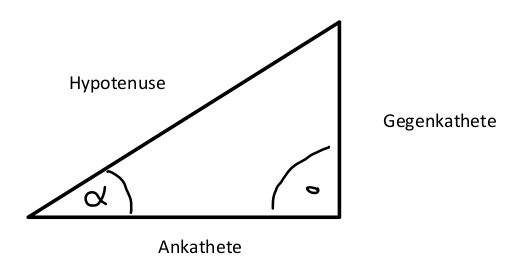
\includegraphics[width=5.5cm]{bild3.png}
\caption{Rechtwinkliges Dreieck}
\end{wrapfigure}
Eselsbrücke
\begin{tabbing}
G~~~~~~\= A~~~~~~\= G~~~~~~\= A \\
\>\>\>\\
H\> H\> A\> G \\
\>\>\>\\
SIN\> COS\> TAN\> COT\\
\end{tabbing}
G = Gegenkathete\\
A = Ankathete\\
H = Hypotenuse
\subsection{Dezimale Vielfache}
\begin{tabular}{|l|l|l|}
\hline
Piko&$p$&$10^{-12}$\\
\hline
Nano&$n$&$10^{-9}$\\
\hline
Mikro&$\mu$&$10^{-6}$\\
\hline
Milli&$m$&$10^{-3}$\\
\hline
Zenti&$c$&$10^{-2}$\\
\hline
Dezi&$d$&$10^{-1}$\\
\hline
&&$10^{-0}$\\
\hline
Deka&$da$&$10^{1}$\\
\hline
Hekto&$h$&$10^{2}$\\
\hline
Kilo&$k$&$10^{3}$\\
\hline
Mega&$M$&$10^{6}$\\
\hline
Giga&$G$&$10^{9}$\\
\hline
Tera&$T$&$10^{12}$\\
\hline
\end{tabular}

\subsection{Quadratische Gleichung}
\begin{description}
\item $ax^{2}+bx+c=0$
\item $x=\frac{-b\pm \sqrt{b^{2}-4ac}}{2a}$
\end{description}

\subsection{Potenzen, Wurzeln, Logarithmen}
\begin{description}
\item $a^{n}=c$
\item $\sqrt[n]{c}=a$
\item $log_{a}c=n$
\item ~~~~$log_{10}c = lg~c~(Zehnerlogarithmus)$
\item ~~~~$log_{e}c ~= ln~c~(Natuerlicher Logarithmus, e=2,781...)$
\item ~~~~$log_{2}c = lb~c~(Zweier Logarithmus)$
\end{description}

\pagebreak
\subsection{Komplexe Zahlen}
\begin{figure}[h]
 \centering
 \includegraphics[width=0.9\textwidth]{"bild5.png"}
 \caption{Komplexe Zahlen}
 \label{fig:komplzahl}
\end{figure}
\begin{description}
\item X Achse (Abszisse) $\Rightarrow$ Realteil a
\item Y Aches (Ordinate) $\Rightarrow$ Imaginärteil b (i Taste auf dem Taschenrechner)
\item $\varphi$ = Winkel zwischen a und b ($\angle$ Taste auf dem Taschenrechner in RAD) 
\end{description}



\pagebreak
\section{Physik}
\subsection{Ohmisches Gesetz}
\subsubsection{Im Gleichstromnetz}
$U = R \cdot I~[V];~~~~R = \frac{U}{I}~[\Omega];~~~~I = \frac{U}{R}~[A]$
\subsection{Leistung}
$P = U \cdot I;~~~~P = I^{2} \cdot R;~~~~P = U^{2} \cdot T~[W]$
\subsubsection{Im Drehstromnetz}
$P = U \cdot I \cdot cos~\varphi \cdot \sqrt{3}~[W]$
\subsubsection{Im Wechselstromnetz}
$P = U \cdot I \cdot cos~\varphi~[W]$
\subsection{Leitungsberechnung}
\begin{description}
\item $A = \frac{2 \cdot l \cdot I \cdot cos~\varphi}{\gamma \cdot \Delta u}$
\item $\Delta u = \frac{2 \cdot l \cdot I \cdot cos~\varphi}{\gamma \cdot A}$
\item $A = \frac{\sqrt{3} \cdot l \cdot I \cdot cos~\varphi}{\gamma \cdot \Delta u}$
\item $\Delta u = \frac{\sqrt{3} \cdot l \cdot I \cdot cos~\varphi}{\gamma \cdot A}$
\end{description}
\subsection{Magnetismus}
Ferromagnetische Stoffe:
\begin{description}
\item Eisen
\item Nickel
\item Cobalt
\end{description}
\subsubsection{Durchflutung}
$\Theta = l \cdot N~~~~\Theta \widehat{=} Theta$
\subsubsection{Feldstärke}
\begin{description}
\item $H \sim \frac{1}{l}~~~~l \widehat{=} $Feldlinienlänge
\item $H = \frac{\Theta}{l}~~~~[\frac{A}{m}]$
\end{description}
\subsubsection{Permeabilität}
\begin{description}
\item $\Phi \sim \mu$
\item $\mu = \mu_{0} \cdot \mu_{r}~~~~r \widehat{=} $relative Permeabilität
\end{description}
\subsubsection{Magnetischer Fluss}
\begin{description}
\item $\Phi \sim A$~~~~Fläche
\item $\Phi \sim H$~~~~Feldstärke
\item $\Phi = \mu \cdot A \cdot H~~~~[Vs] = [Wb] Weber ~~~~ \Phi \widehat{=} Phi$
\end{description}

\subsubsection{Magnetischer Flussdichte}
\begin{description}
\item $B = \frac{\Phi}{A}~~~~[\frac{Vs}{mm^{2}}]=[T]Tesla$
\item $B = \mu \cdot H$
\item $\mu = \frac{B}{H}~~~~[\frac{Vs}{Am}]$
\end{description}
\subsubsection{Magnetische Feldkonstante}
\begin{description}
\item $\mu_{0} = 4 \cdot  \pi \cdot 10 ^{-7}~~~~[Am]$
\item $\mu_{0} = 1,257 \cdot 10 ^{-6}~~~~[Am]$
\end{description}
\subsection{Gleichstrom}
\subsection{Wechselstrom}
\begin{description}
\item $U=Z \cdot I$
\item $P=U \cdot I \cdot cos \varphi$
\item $S=U \cdot I$
\item $Z=\sqrt{R^{2}+X^{2}}$
\item ~~~~$R \widehat{=} Wirkwiderstand$
\item ~~~~$X \widehat{=} Blindwiderstand$
\item ~~~~$Z \widehat{=} Scheinwiderstand$
\item $S=\sqrt{P^{2}+Q^{2}}$
\item ~~~~$P \widehat{=} Wirkleistung [W]$
\item ~~~~$Q \widehat{=} Blindleistung [var]$
\item ~~~~$S \widehat{=} Scheinleistung [VA]$
\item $cos \varphi = \frac{R}{Z}$
\item $X_{L} = 2 \cdot \pi \cdot f \cdot L$
\item $X_{C} = \frac{1}{2 \cdot \pi \cdot f \cdot C} $
\end{description}
\subsection{Drehstrom}
\begin{description}
\item $S = U \cdot I \cdot \sqrt{3} \cdot cos \varphi$
\item $P = U \cdot I \cdot cos \varphi$
\end{description}
\subsection{Kondensator}



\end{document}